% !TeX program = xelatex
% 中文期刊论文：按照南方电网技术投稿要求改写
% 编译建议：XeLaTeX。中文字体优先使用系统字体，缺失时回退到 TeX Live/CTeX 常见的 Fandol 字体。
\documentclass[UTF8,zihao=5,twoside]{ctexart}

\usepackage[a4paper,top=22mm,bottom=20mm,left=18mm,right=18mm,headheight=14pt,headsep=6mm,columnsep=7mm]{geometry}
\usepackage{fontspec}
\usepackage{xeCJK}
\usepackage{amsmath,amssymb,bm}
\usepackage{graphicx}
\usepackage{float}
\usepackage{booktabs,array,multirow,tabularx}
\usepackage{caption}
\usepackage{titlesec}
\usepackage{fancyhdr}
\usepackage{indentfirst}
\usepackage{enumitem}
\usepackage{multicol}
\usepackage{balance}
\usepackage{tikz}
\usetikzlibrary{arrows.meta,positioning,shapes.geometric}
\usepackage[hidelinks]{hyperref}

\graphicspath{{figures/}}

% -------------------- 字体 --------------------
\IfFontExistsTF{Songti SC}
  {\setCJKmainfont{Songti SC}}
  {\IfFontExistsTF{SimSun}
    {\setCJKmainfont{SimSun}}
    {\setCJKmainfont{FandolSong-Regular.otf}[BoldFont=FandolSong-Bold.otf,ItalicFont=FandolKai-Regular.otf]}}
\IfFontExistsTF{Heiti SC}
  {\setCJKsansfont{Heiti SC}}
  {\IfFontExistsTF{SimHei}
    {\setCJKsansfont{SimHei}}
    {\setCJKsansfont{FandolHei-Regular.otf}[BoldFont=FandolHei-Bold.otf]}}
\IfFontExistsTF{Kaiti SC}
  {\setCJKfamilyfont{kai}{Kaiti SC}}
  {\IfFontExistsTF{KaiTi}
    {\setCJKfamilyfont{kai}{KaiTi}}
    {\setCJKfamilyfont{kai}{FandolKai-Regular.otf}}}
\IfFontExistsTF{Times New Roman}{\setmainfont{Times New Roman}}{\IfFontExistsTF{TeX Gyre Termes}{\setmainfont{TeX Gyre Termes}}{\setmainfont{Latin Modern Roman}}}
\IfFontExistsTF{Arial}{\setsansfont{Arial}}{\IfFontExistsTF{TeX Gyre Heros}{\setsansfont{TeX Gyre Heros}}{\setsansfont{Latin Modern Sans}}}
\newcommand{\kaiti}{\CJKfamily{kai}}

\zihao{5}
\setlength{\parindent}{2em}
\linespread{1.08}
\setlist{nosep,leftmargin=2em}
\setlength{\textfloatsep}{0.7em plus 0.2em minus 0.2em}
\setlength{\floatsep}{0.6em plus 0.2em minus 0.2em}
\setlength{\intextsep}{0.6em plus 0.2em minus 0.2em}
\renewcommand{\topfraction}{0.95}
\renewcommand{\bottomfraction}{0.85}
\renewcommand{\textfraction}{0.05}
\renewcommand{\floatpagefraction}{0.85}
\setcounter{topnumber}{4}
\setcounter{bottomnumber}{2}
\setcounter{totalnumber}{6}

% -------------------- 页眉页脚 --------------------
\pagestyle{fancy}
\fancyhf{}
\fancyhead[LE]{\zihao{-5}第~\thepage~页}
\fancyhead[CE]{\zihao{-5}南方电网技术}
\fancyhead[RE]{\zihao{-5}第~XX~卷}
\fancyhead[LO]{\zihao{-5}\thepage}
\fancyhead[CO]{\zihao{-5}南方电网技术}
\fancyhead[RO]{\zihao{-5}第~XX~卷}
\renewcommand{\headrulewidth}{0.4pt}
\renewcommand{\footrulewidth}{0pt}

% -------------------- 标题层级 --------------------
\titleformat{\section}{\sffamily\zihao{4}\bfseries}{\thesection}{0.6em}{}
\titleformat{\subsection}{\sffamily\zihao{5}\bfseries}{\thesubsection}{0.6em}{}
\titleformat{\subsubsection}{\sffamily\zihao{5}\bfseries}{\thesubsubsection}{0.6em}{}
\titlespacing*{\section}{0pt}{0.8em}{0.4em}
\titlespacing*{\subsection}{0pt}{0.6em}{0.3em}
\titlespacing*{\subsubsection}{0pt}{0.4em}{0.2em}

% -------------------- 图表与公式 --------------------
\captionsetup{font={small},labelfont=bf,labelsep=quad,justification=centering}
\renewcommand{\figurename}{图}
\renewcommand{\tablename}{表}
\numberwithin{equation}{section}
\renewcommand{\theequation}{\arabic{equation}}

\newcommand{\figbicaption}[2]{%
  \caption{#1\\[-0.2em]\small Fig.\,\thefigure\ #2}
}
\newcommand{\tabbicaption}[2]{%
  \caption{#1\\[-0.2em]\small Tab.\,\thetable\ #2}
}
\newcommand{\metric}[1]{\mathrm{#1}}
\newcommand{\code}[1]{\texttt{#1}}

% -------------------- 参考文献格式 --------------------
\renewcommand{\refname}{参考文献}
\makeatletter
\renewenvironment{thebibliography}[1]{%
  \section*{\refname}%
  \small
  \list{[\arabic{enumi}]}{%
    \settowidth\labelwidth{[#1]}%
    \leftmargin\labelwidth
    \advance\leftmargin\labelsep
    \usecounter{enumi}}
  \sloppy\clubpenalty4000\widowpenalty4000\sfcode`\.\ \@m
}{\def\@noitemerr{\@latex@warning{Empty `thebibliography' environment}}\endlist}
\makeatother

\newcommand{\articleinfo}{文章编号：1674-0629(20XX)XX-XXXX-XX\quad 中图分类号：TM73\quad 文献标志码：A\\
DOI：10.13648/j.cnki.issn1674-0629.20XX.XX.XXX}

\newcommand{\fundcn}{基金项目：无。}
\newcommand{\funden}{Foundation item: None.}

\begin{document}
\twocolumn[

% ==================== 首页题名与摘要：单栏 ====================
\begin{center}
{\zihao{-5}\articleinfo}\par\vspace{1.0em}
{\sffamily\zihao{2}\bfseries 基于多相关性筛选与 L1 门控深度神经网络的电力数据隐性推断风险分析}\par\vspace{0.8em}
{\zihao{4}杜浩存}\par\vspace{0.4em}
{\zihao{5}（西安交通大学 网络空间安全学院，陕西 西安 710049）}\par\vspace{0.8em}
\end{center}

\noindent\textbf{摘要：}电力系统运行与市场数据由物理约束、调度策略和市场出清机制共同生成，字段之间存在复杂且稳定的统计关联。在数据开放共享场景下，攻击者可利用公开的低敏感字段组合推断高敏感目标字段，构成隐性推断风险。针对传统相关性分析无法刻画联合推断能力、全量深度模型无法定位关键风险源字段的问题，提出了一种融合多相关性筛选与 L1 门控深度神经网络的隐性推断风险分析方法。首先，利用 Pearson、Spearman、Kendall 相关系数以及归一化互信息、距离相关系数和 HSIC 六类统计指标，对候选字段进行多维度依赖性初筛；然后，在深度神经网络输入端引入可学习门控向量，并施加 L1 正则化约束实现冗余字段压缩，获取能够维持敏感目标推断能力的紧凑推断源集合；此外，构建了相关性驱动的改进门控模型，将六类统计指标映射为统一的风险判定边界。基于美国 PJM 电力市场 2025 年小时级运行数据开展实验，结果表明：以净实际交换功率为目标，L1 门控从 55 个候选字段中筛选出 18 个活跃字段，以此训练的普通深度神经网络验证 $R^2$ 达到 0.9681，高于全量 55 字段的 0.9661，而未选中字段单独推断仅为 0.7820；在 12 个敏感目标上，L1 门控模型平均使用 15.5 个字段，字段利用率约为 22.46\%，平均测试 $R^2$ 为 0.9111，高于全量模型的 0.9031。同预算对比和冗余噪声分析实验进一步验证了所提方法在字段压缩、推断能力保持与风险解释方面的有效性。\par
\noindent\textbf{关键词：}电力数据安全；隐性推断风险；相关性分析；L1 门控神经网络；特征选择；数据共享\par\vspace{0.8em}

\begin{center}
{\bfseries\large Implicit Inference Risk Analysis for Power Data Based on Multi-Correlation Screening and L1-Gated Deep Neural Network}\par\vspace{0.5em}
{DU Haocun}\par\vspace{0.3em}
{\small (School of Cyber Science and Engineering, Xi'an Jiaotong University, Xi'an 710049, China)}\par\vspace{0.5em}
\end{center}

\noindent\textbf{Abstract:} Power system operation and market data are jointly shaped by physical constraints, dispatching strategies and market clearing mechanisms, giving rise to complex and stable statistical dependencies among data fields. In data sharing scenarios, adversaries may exploit combinations of publicly available low-sensitivity fields to infer high-sensitivity targets, thereby creating implicit inference risks. To address the limitations of conventional correlation analysis in characterizing joint inference capability and the inability of full-feature deep models to locate critical risk-source fields, this paper proposes an implicit inference risk analysis method that integrates multi-correlation screening with an L1-gated deep neural network. Six statistical dependency measures, namely Pearson, Spearman, Kendall correlation coefficients, normalized mutual information, distance correlation, and HSIC, are first employed for multi-dimensional candidate screening. A learnable gate vector is then inserted at the DNN input layer, and L1 regularization is applied to compress redundant fields and obtain a compact inference-source set that preserves prediction capability for sensitive targets. Furthermore, a correlation-driven improved gate model is constructed to map the six statistical measures into a unified risk boundary. Experiments conducted on the 2025 PJM hourly market data demonstrate that, for net actual interchange, the L1 gate selects 18 active features from 55 candidates, with a standard DNN retrained on these features achieving a test $R^2$ of 0.9681, compared with 0.9661 for all features and 0.7820 for unselected features alone. Across 12 sensitive targets, the L1-gated model uses 15.5 features on average with a usage ratio of 22.46\% and an average test $R^2$ of 0.9111, exceeding 0.9031 for the full-feature model. Same-budget baseline comparisons and redundant-noise analysis experiments further validate the effectiveness of the proposed method in field compression, inference preservation, and risk interpretation.\par
\noindent\textbf{Key words:} power data security; implicit inference risk; correlation analysis; L1-gated neural network; feature selection; data sharing\par\vspace{0.8em}

\noindent{\small\fundcn\\\funden}
\vspace{0.8em}
]

\section{引言}
随着新型电力系统建设和电力市场化改革的不断深入，调度控制、市场交易、负荷预测、辅助服务和交换功率等各环节持续产生海量结构化数据\cite{ref-liu-cps,ref-ma-pjm}。电力数据的开放共享对于支撑电网运行分析、市场监管、学术研究和算法验证具有重要意义\cite{ref-fan-pjm}。然而，电力系统作为典型的信息物理融合系统，其运行状态受到潮流平衡方程、设备物理约束、调度策略和市场出清规则的共同约束，不同字段之间天然形成了稳定且具有明确物理含义的统计关联。这种内在关联结构在数据开放共享场景下可能引发新的安全风险。

关于电力数据隐私与安全，国内外已有大量研究。智能电表隐私保护方面，文献\cite{ref-sankar}从信息论角度构建了智能电表隐私框架，证明细粒度用电数据可被用于推断用户行为；文献\cite{ref-giaconi}综述了智能计量系统的隐私保护进展和挑战；文献\cite{ref-adewole}则分析了能源分解技术可能带来的数据泄露风险。上述研究表明，攻击者可以利用合法获取或公开发布的数据恢复更高敏感度的信息。然而，已有研究主要关注终端用电数据的隐私推断，对于电网运行和市场层面的多字段联合推断风险尚缺乏系统性研究。

在相关性分析与特征选择方面，Pearson 相关系数、Spearman 和 Kendall 秩相关系数已广泛应用于负荷预测和数据清洗中的特征筛选\cite{ref-lan-load,ref-jiao-pv,ref-deng-load}。为刻画变量间的非线性依赖关系，距离相关系数\cite{ref-szekely-dcorr}和 HSIC\cite{ref-gretton-hsic}等核方法也被引入电力数据分析领域。然而，上述方法存在两方面不足：其一，单一统计指标仅能捕捉特定数学意义下的依赖关系，在面对电力数据中既有线性又有非线性耦合的复杂场景时容易产生遗漏；其二，统计相关性强弱不能直接等价于联合推断模型中字段的重要性，相关性弱的字段在组合后仍可能提供有效的互补信息。

基于机器学习的推断建模方法为验证字段间推断能力提供了另一条途径。深度神经网络、随机森林\cite{ref-breiman-rf}和 XGBoost\cite{ref-chen-xgboost}等模型已在电力数据分析中得到广泛应用\cite{ref-wang-meter}。这类方法能够直接验证目标字段是否可由其余字段恢复，但全量深度模型仅能给出整体可预测性判断，难以回答"哪些字段构成主要风险源"这一关键问题。Lasso\cite{ref-tibshirani-lasso}和 ElasticNet\cite{ref-zou-enet}等稀疏线性模型虽具有变量选择功能，但其表达能力受限于线性假设；树模型的特征重要性排序则容易受到特征冗余和训练随机性的干扰。文献\cite{ref-xing-micdnn}提出的 MIC-DNN 框架将信息系数与深度模型相结合用于电力数据相关性验证，但该方法局限于成对推断，难以识别多字段联合场景下的非冗余推断源集合。

综上所述，面向电力数据发布前安全审查的隐性推断风险分析，需要同时满足三方面要求：一是充分捕捉不同类型的统计依赖关系，避免潜在风险字段的过早遗漏；二是验证字段集合对敏感目标的实际推断能力，而非停留在统计指标层面；三是在保持推断能力的前提下最大程度压缩冗余字段，使分析结果能够精确定位到具体的风险源字段，为后续的字段级安全处置提供依据。基于上述分析，本文提出了融合多相关性筛选与 L1 门控深度神经网络的电力数据隐性推断风险分析方法，主要贡献如下：

1）提出了多相关性初筛与 L1 门控深度神经网络相结合的隐性推断风险分析框架，将多类型统计依赖证据、非线性推断能力验证和字段稀疏选择统一到同一分析流程中。

2）针对净实际交换功率目标开展了单目标细粒度实验，通过门控参数演化分析、活跃字段数量变化追踪和 Top-n 再训练验证，揭示了所选字段集合的充分推断能力和未选中字段的冗余特性。

3）在 12 个敏感目标上开展了全量模型与 L1 门控模型的系统对比，并设计了 95\% 和 97\% 同预算 baseline 对比实验，验证了所提方法在相同字段预算约束下相较单相关性选择、线性稀疏模型和树模型重要性排序的综合优势。

4）针对少量字段推断精度高于全量字段的现象进行了冗余噪声影响分析，通过训练曲线对比和 Top-n 递增实验，阐明了全量输入中冗余字段引发过拟合的机理，为合理的字段压缩策略提供了理论依据。

\section{隐性推断风险分析方法}
\subsection{问题定义与总体流程}
在电力数据开放共享场景中，敏感字段并不一定以明文形式直接发布，但其取值可能由若干低敏感字段共同推断得到。与传统的数据脱敏问题不同，隐性推断风险关注的是字段之间的联合可恢复性：即攻击者是否能够利用已公开字段构造推断模型，从而恢复原本不应暴露的目标字段。给定电力数据集
\begin{equation}
D=\{X_1,X_2,\ldots,X_w,Y\},
\end{equation}
其中 $Y\in\mathbb{R}^{n}$ 为待保护的敏感目标字段，$X_i\in\mathbb{R}^{n}$ 为候选字段，$w$ 为候选字段总数，$n$ 为样本数。本文将隐性推断风险分析定义为：在候选字段空间中识别一个规模尽可能小的字段集合 $\mathcal{S}$，使其仍能对敏感目标 $Y$ 保持较高推断能力，即
\begin{equation}
\mathcal{S}^{*}=\arg\min_{\mathcal{S}\subseteq \{X_i\}}\left|\mathcal{S}\right|,
\quad
R^2(f_{\theta}(\mathcal{S}),Y)\geq \eta .
\end{equation}
式中：$f_{\theta}$ 为推断模型；$\eta$ 为可接受的推断能力阈值。模型推断性能采用决定系数 $R^2$ 衡量：
\begin{equation}
R^2=1-\frac{\sum_{k=1}^{n}(y_k-\hat{y}_k)^2}{\sum_{k=1}^{n}(y_k-\bar{y})^2}.
\end{equation}
式中：$y_k$ 为真实值；$\hat{y}_k$ 为模型预测值；$\bar{y}$ 为真实值的均值。若一个较小字段集合取得的 $R^2$ 接近或超过全量字段结果，说明该集合保留了主要推断路径；若被剔除字段单独推断能力明显下降，则说明这些字段主要提供冗余信息或噪声。

围绕上述定义，本文方法并不直接以全量字段训练一个黑箱预测模型，而是按照"统计依赖发现--推断模型验证--稀疏风险定位--相关性权重解释"的思路展开。首先，通过多类相关性指标对候选字段进行宽松初筛，保留可能与目标存在显著统计依赖的字段；其次，在初筛后的候选空间中训练 L1 门控深度神经网络，使模型在保持预测能力的同时压缩冗余字段；最后，利用相关性驱动的改进门控模型学习不同相关性证据对推断风险的贡献权重，形成统一的风险判定边界。整体流程如图~\ref{fig:method_flow} 所示。

\begin{figure}[!tbp]
\centering
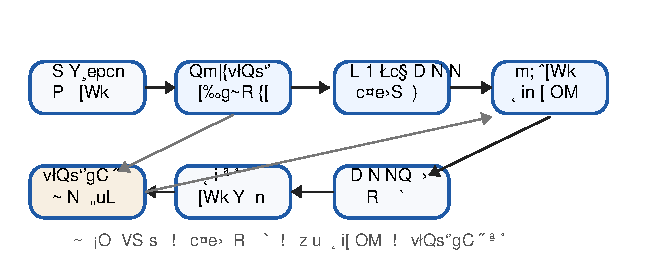
\includegraphics[width=\columnwidth]{method_flow.pdf}
\figbicaption{隐性推断风险分析总体流程}{Overall workflow of implicit inference risk analysis}
\label{fig:method_flow}
\end{figure}

该流程的关键在于将"是否相关"与"是否能够用于推断"区分开来。相关性分析适合快速发现候选依赖关系，但难以直接回答字段组合在非线性模型中的实际作用；深度推断模型能够验证目标字段的可恢复性，但全量模型难以定位具体风险源。本文通过两者结合，使初筛阶段具有充分覆盖性，使门控阶段具有推断导向性，并使最终输出能够服务于字段级安全审查。

\subsection{多相关性初筛}
相关系数是分析变量关联关系的常用统计工具，其基本思想是将两个变量之间的同步变化、单调变化或分布依赖压缩为一个标量指标，从而快速判断字段之间是否存在潜在联系。在电力数据分析中，相关性方法常用于负荷预测特征选择、异常数据清洗和运行变量筛查等任务\cite{ref-lan-load,ref-jiao-pv,ref-deng-load}。然而，电力系统数据由物理约束、调度规则和市场机制共同生成，字段之间既可能存在近似线性关系，也可能存在排序一致但非线性的单调关系，还可能体现为复杂的分布依赖或核空间依赖。因此，单一相关系数往往只能覆盖某一种关联形态，容易在初筛阶段遗漏潜在风险字段。

为提高候选字段覆盖能力，本文从线性相关、秩相关、信息论相关和核相关四个角度构建六维相关性向量：
\begin{equation}
R_i=[r_i^{(\metric{NMI})},r_i^{(\metric{Spear})},r_i^{(\metric{Pear})},
r_i^{(\metric{Ken})},r_i^{(\metric{DC})},r_i^{(\metric{HSIC})}].
\end{equation}
式中：六个分量分别为归一化互信息（NMI）、Spearman 秩相关系数、Pearson 相关系数、Kendall 秩相关系数、距离相关系数（DC）和 Hilbert-Schmidt 独立性准则（HSIC）。

Pearson 相关系数用于度量两个变量之间的线性相关程度，其形式为
\begin{equation}
r^{(\metric{Pear})}(X,Y)=
\frac{\sum_{k=1}^{n}(x_k-\bar{x})(y_k-\bar{y})}
{\sqrt{\sum_{k=1}^{n}(x_k-\bar{x})^2}\sqrt{\sum_{k=1}^{n}(y_k-\bar{y})^2}} .
\end{equation}
当电力字段之间近似满足线性耦合关系时，如部分负荷、发电量和交换功率字段，Pearson 指标能够直接反映其线性联动强度。Spearman 相关系数则先将变量值转换为秩次，再计算秩次之间的 Pearson 相关：
\begin{equation}
r^{(\metric{Spear})}(X,Y)=r^{(\metric{Pear})}(\metric{rank}(X),\metric{rank}(Y)).
\end{equation}
该指标对非线性单调关系更敏感，能够捕捉"数值变化不线性但排序趋势一致"的依赖关系。Kendall 秩相关系数从样本对的一致性角度度量单调依赖：
\begin{equation}
r^{(\metric{Ken})}(X,Y)=\frac{N_c-N_d}{n(n-1)/2},
\end{equation}
式中：$N_c$ 和 $N_d$ 分别为一致样本对和不一致样本对数量。与 Spearman 相比，Kendall 更强调样本排序方向的一致性，适合对排序扰动较敏感的关系判断。

归一化互信息从信息论角度衡量变量之间共享信息量\cite{ref-cover-info}，其定义为
\begin{equation}
r^{(\metric{NMI})}(X,Y)=\frac{I(X;Y)}{\sqrt{H(X)H(Y)}} .
\end{equation}
式中：$I(X;Y)$ 为互信息；$H(X)$ 和 $H(Y)$ 为信息熵。该指标不要求变量之间满足线性或单调假设，适合发现一般非线性统计依赖。距离相关系数通过样本间距离矩阵度量变量之间的依赖关系\cite{ref-szekely-dcorr}，当且仅当两个变量独立时其理论值为零，因而可以作为非线性依赖的补充证据。HSIC 则将变量映射到再生核 Hilbert 空间中，通过交叉协方差算子的 Hilbert-Schmidt 范数刻画依赖强度\cite{ref-gretton-hsic}，在复杂非线性关系识别中具有较强表达能力。

六类指标的作用并非简单重复，而是形成互补的风险证据集合。Pearson 关注线性同涨同落，Spearman 和 Kendall 关注排序一致性，NMI 关注信息共享，DC 和 HSIC 关注更一般的非线性依赖。对于电力市场数据而言，同一目标字段的推断路径可能同时包含物理线性约束、市场出清导致的分段关系以及燃料结构引起的非线性耦合，因此需要多指标联合初筛以降低漏检风险。

本文将初筛定位为候选空间压缩，而非最终风险判定。具体流程如图~\ref{fig:corr_screening_flow} 所示：首先分别计算每个候选字段与敏感目标之间的六类相关性指标；然后对不同指标进行归一化和阈值判断；最后采用"任一指标通过即保留"的宽松规则生成候选字段集合：
\begin{equation}
q_i=\max_j I\left(r_i^{(j)}\geq \mu_1^{(j)}\right),
\quad
X_i\in\mathcal{C}\ \mathrm{if}\ q_i=1 .
\end{equation}
式中：$I(\cdot)$ 为示性函数；$\mu_1^{(j)}$ 为第 $j$ 类指标的初筛阈值；$\mathcal{C}$ 为进入门控模型的候选字段集合。宽松规则的设计依据是：初筛阶段宁可保留少量冗余字段，也不应过早删除潜在推断源；字段的最终取舍由后续 L1 门控模型在推断训练中完成。

\begin{figure}[!tbp]
\centering
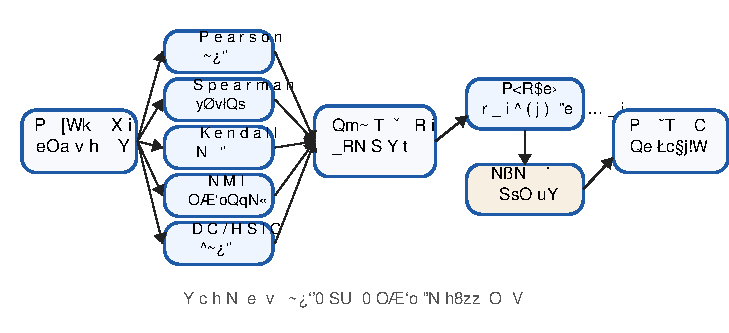
\includegraphics[width=\columnwidth]{corr_screening_flow.pdf}
\figbicaption{多相关性初筛流程}{Workflow of multi-correlation screening}
\label{fig:corr_screening_flow}
\end{figure}

\subsection{L1 门控深度推断模型}
多相关性初筛能够发现统计依赖，但相关性强并不必然意味着字段在联合推断模型中不可替代。一个字段可能与目标高度相关，却被另一个字段完全覆盖；也可能单独相关性不强，但与其他字段组合后提供关键互补信息。因此，初筛之后仍需要一个推断导向的选择机制，在实际预测任务中判断字段是否真正参与敏感目标恢复。为此，本文在深度神经网络输入端引入可学习门控层，构建 L1 门控深度推断模型。

设初筛得到的候选字段集合为 $X=\{X_1,\ldots,X_m\}$，其中 $m$ 为通过初筛的字段数。门控层为每个输入字段分配一个可学习参数 $g_i$，并在进入神经网络前对输入进行逐元素加权：
\begin{equation}
\tilde{X}=g\odot X,\quad g=[g_1,g_2,\ldots,g_m].
\end{equation}
随后，$\tilde{X}$ 被输入到多层全连接网络中，得到敏感目标的预测值：
\begin{equation}
\hat{Y}=f_{\theta}(\tilde{X})=f_{\theta}(g\odot X).
\end{equation}
模型结构如图~\ref{fig:l1_gate_structure} 所示。与普通 DNN 直接接收全部字段不同，门控 DNN 在输入端显式设置了字段选择通道，使每个字段是否被模型使用可以通过门控参数的大小进行解释。

\begin{figure*}[!t]
\centering
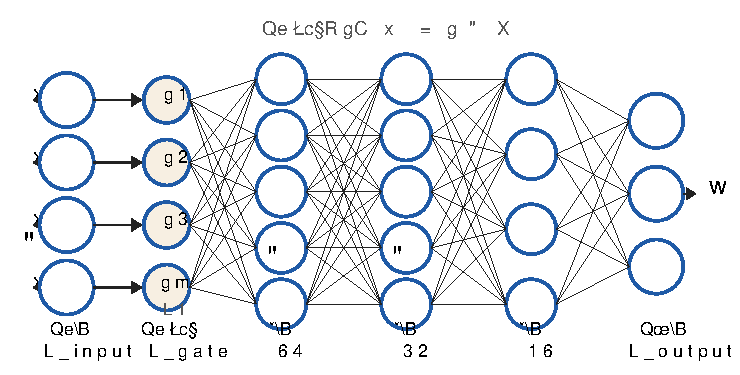
\includegraphics[width=0.92\textwidth]{l1_gate_structure.pdf}
\figbicaption{L1 门控深度推断模型结构}{Structure of the L1-gated deep inference model}
\label{fig:l1_gate_structure}
\end{figure*}

为了使门控参数具有稀疏选择能力，本文在预测损失之外加入 L1 正则项，训练目标为
\begin{equation}
\mathcal{L}=\frac{1}{n}\sum_{k=1}^{n}(y_k-\hat{y}_k)^2+\lambda\sum_{i=1}^{m}|g_i|.
\end{equation}
式中：第一项为均方误差损失，用于保证模型对敏感目标的推断能力；第二项为门控参数的 L1 惩罚，$\lambda$ 为正则化系数。L1 正则化具有推动参数稀疏化的作用：若某字段对降低预测误差具有稳定贡献，反向传播会抵消正则惩罚并维持其较大门控值；若某字段仅提供冗余或噪声，L1 惩罚会持续压低其门控值，使其逐渐接近零。

训练结束后，本文根据门控参数大小识别活跃推断源：
\begin{equation}
|g_i|\geq \mu_2 .
\end{equation}
式中：$\mu_2$ 为活跃阈值。满足条件的字段构成活跃字段集合 $\mathcal{S}$。与单纯的特征重要性排序不同，门控参数是在预测损失和稀疏约束的共同作用下形成的，因此其含义更接近"该字段是否被推断模型实际利用"。为避免门控模型自身结构对结果产生偶然影响，本文进一步使用普通 DNN 在 $\mathcal{S}$ 上重新训练并评估 $R^2$，将再训练结果作为所选字段集合推断能力的独立验证。本文将活跃字段数量记为 $n_s$，并在后续同预算对比实验中作为统一字段预算，使不同选择方法在相同字段数量下比较字段选择质量。

\subsection{相关性驱动的改进门控}
普通 L1 门控模型能够在推断任务中识别关键字段，但每个字段的门控参数是独立学习得到的，无法直接说明六类相关性证据分别对推断风险贡献了多少。另一方面，多相关性初筛虽然提供了丰富的统计依赖信息，但其作用仍主要停留在描述性筛查层面：相关系数被用于判断字段是否进入候选集合，却没有进一步嵌入推断模型，也没有形成一个能够统一融合不同相关性指标的判定函数。因此，初筛和推断之间仍存在一定割裂。

在实际数据发布审查中，还常常会遇到新增字段快速评估的问题。假设新增加一列数据 $X_{\mathrm{new}}$，若每次都重新训练完整门控模型，计算成本较高，也不利于发布流程中的快速预审。更理想的方式是：先计算 $X_{\mathrm{new}}$ 与敏感目标 $Y$ 的六类相关性向量，再根据各类相关性指标对最终推断风险的贡献权重，直接得到一个敏感度评分。基于这一考虑，本文提出相关性驱动的改进门控思路，将六维相关性向量作为门控输入，用可学习权重刻画不同相关性指标对推断风险的相对贡献。

对于字段 $X_i$，改进门控不再为其设置独立自由参数，而是由六维相关性向量 $R_i$ 生成门控值：
\begin{equation}
g_i=\sigma(W^{\mathrm{T}}R_i+b),
\end{equation}
式中：$W\in\mathbb{R}^{6}$ 为六类相关性指标对应的可学习权重向量；$b$ 为偏置项；$\sigma(\cdot)$ 为 Sigmoid 激活函数，其定义为
\begin{equation}
\sigma(z)=\frac{1}{1+\exp(-z)} .
\end{equation}
Sigmoid 函数将任意实数映射到 $(0,1)$ 区间，可将线性融合得分解释为字段门控打开程度或风险敏感度。其函数在 $z=0$ 处取值为 0.5，当 $z$ 增大时输出逐渐接近 1，表示相关性证据更支持字段作为推断源；当 $z$ 减小时输出逐渐接近 0，表示字段更可能为低贡献或冗余字段。由此可得，改进门控天然给出门控开闭的中性阈值：
\begin{equation}
W^{\mathrm{T}}R_i+b=0
\quad \Longleftrightarrow \quad
g_i=0.5 .
\end{equation}
因此，$g_i=0.5$ 不再是人工指定的经验阈值，而是 Sigmoid 函数中心点对应的自然边界。当 $g_i>0.5$ 时，字段位于风险边界上方；当 $g_i<0.5$ 时，字段位于风险边界下方。该边界将六类相关性指标统一到同一判定平面中，使不同统计证据不再各自孤立地发挥作用。

改进门控的结构如图~\ref{fig:corr_gate_structure} 所示。与普通 L1 门控直接学习每个字段的独立门控值不同，改进门控先将字段与目标之间的六类相关性组织为 $R_i$，再通过 $W^{\mathrm{T}}R_i+b$ 完成加权融合，并经 Sigmoid 函数得到 $g_i$。因此，门控值不仅表示字段是否被打开，也携带了不同相关性指标对该字段风险判定的贡献信息。

\begin{figure*}[!t]
\centering
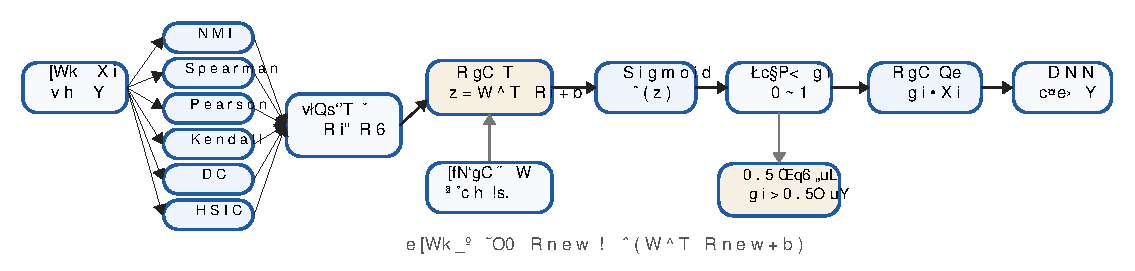
\includegraphics[width=0.96\textwidth]{corr_gate_structure.pdf}
\figbicaption{相关性驱动改进门控结构}{Structure of the correlation-driven improved gate}
\label{fig:corr_gate_structure}
\end{figure*}

改进门控的训练目标仍由预测损失和稀疏惩罚构成，但正则化对象从独立门控参数转变为由相关性向量生成的门控值：
\begin{equation}
\mathcal{L}_{\mathrm{cg}}=
\frac{1}{n}\sum_{k=1}^{n}(y_k-\hat{y}_k)^2
+\lambda\sum_{i=1}^{m}\sigma(W^{\mathrm{T}}R_i+b).
\end{equation}
在训练过程中，预测误差驱动模型提高有助于目标恢复的字段门控值，L1 型稀疏约束则压低贡献不足的字段门控值。训练完成后，权重向量 $W$ 的各分量反映了不同相关性指标在该敏感目标推断任务中的相对贡献。例如，若 HSIC 对应权重较大，说明核空间非线性依赖在该目标的风险判定中更重要；若 Pearson 权重较大，则说明线性耦合对该目标的恢复更具解释力。

与普通 L1 门控相比，相关性驱动门控的主要价值不在于单纯追求更高 $R^2$，而在于将统计依赖证据转化为推断导向的融合边界。一方面，它提高了模型解释性，使研究者能够观察不同相关系数在风险判断中的权重；另一方面，它为新增字段的快速预审提供了可能：对于新字段，只需计算其与目标字段的六维相关性向量 $R_{\mathrm{new}}$，即可通过 $\sigma(W^{\mathrm{T}}R_{\mathrm{new}}+b)$ 获得风险敏感度评分，而不必立即重新训练完整深度模型。对于数据发布前的批量字段审查而言，这种机制能够在保持推断导向的同时降低重复训练成本。

\section{实验设置}
\subsection{数据集}
实验数据采用美国 PJM 互联电网 2025 年小时级市场与运行数据，数据路径为 \code{NEW\_PROJECT/data/processed/data2025\_Processed\_V2/}。该数据集包含 8760 行（对应全年逐小时记录）和 72 列，其中前两列为 UTC 和东部时间的时间戳，仅用于时间对齐，不参与建模分析。去除时间字段后，剩余 70 个数据字段可按照 PJM Data Miner 官方数据源定义划分为如表~\ref{tab:data_overview} 所示的类别。数据涵盖发电与损耗、风电光伏出力、燃料类型发电、负荷预测与计量、调频市场、辅助服务市场、节点电价和交换功率等多个业务领域，字段间存在广泛的物理和市场机制关联。

\begin{table}[!tbp]
\centering
\scriptsize
\setlength{\tabcolsep}{2pt}
\tabbicaption{PJM 2025 数据字段分类概览}{Classification of PJM 2025 data fields}
\label{tab:data_overview}
\begin{tabularx}{\columnwidth}{c>{\raggedright\arraybackslash}p{0.40\columnwidth}X}
\toprule
编号 & Dataset & 中文说明 \\
\midrule
D1--D2 & Generation and EHV Losses & 小时级总发电量与超高压损耗数据。 \\
D3 & Wind Generation & PJM 区域小时级风电出力。 \\
D4 & Solar Generation & PJM 区域小时级光伏出力。 \\
D5--D24 & Generation by Fuel Type & 按燃料类型统计的发电出力与占比。 \\
D25--D26 & Historical Load Forecasts & 日前及最新可用负荷预测。 \\
D27 & Hourly Load: Preliminary & 由遥测数据计算的预估小时负荷。 \\
D28 & Hourly Load: Metered & PJM RTO 服务区域计量负荷。 \\
D29--D37 & Regulation Billing Data & 调频市场预结算相关价格、容量与信用数据。 \\
D38--D56 & Day-Ahead AS Market Results & 日前辅助服务市场的价格、需求与容量结果。 \\
D57--D60 & Day-Ahead Hourly LMPs & 日前能量市场 LMP、拥塞价与边际损耗价。 \\
D61--D64 & Real-Time Hourly LMPs & 实时能量市场 LMP、拥塞价与边际损耗价。 \\
D65--D70 & Actual/Schedule Summary & 净/总实际、计划和非计划交换功率。 \\
\bottomrule
\end{tabularx}
\end{table}

\subsection{参数设置}
多相关性初筛阶段的各项阈值设置如下：归一化互信息（NMI）为 0.06、Spearman 秩相关系数为 0.15、Pearson 相关系数为 0.15、Kendall 秩相关系数为 0.12、距离相关系数为 0.20、HSIC 为 0.25。上述阈值均用于"任一指标通过即保留"的宽松初筛规则。深度神经网络主干结构采用三层全连接隐藏层，各层神经元数量依次为 64、32 和 16；优化器采用 Adam；批次大小设为 50；训练轮数为 200；随机种子固定为 42 以保证实验可重复性。普通 L1 门控模型的 L1 正则化系数 $\lambda$ 设为 0.002，活跃阈值 $\mu_2$ 设为 0.10。改进 L1 门控模型的门控判定阈值为 0.50，L1 正则化系数设为 0.016，权重向量 $W$ 和偏置 $b$ 分别配置独立学习率，以确保相关性权重和风险偏置的稳定收敛。

\subsection{对比方法}
为全面评估所提方法的有效性，本文设计了三组对比实验。

第一组为全量模型与 L1 门控模型的直接对比。全量 DNN 使用当前目标允许的全部候选字段进行训练，L1DNN 则先由 L1 门控模型获取活跃字段集合，再以相同的 DNN 结构重新训练并评估推断性能。该组对比旨在验证 L1 门控在字段压缩后是否仍能保持甚至提升推断能力。

第二组为同预算 baseline 对比。具体而言，先利用 L1 门控模型在不同特征预算序列上搜索，确定使其 $R^2$ 达到全量 DNN 的 95\% 或 97\% 水平时所需的字段数 $n$；随后分别采用 NMI、Pearson、Spearman 排序选择、Lasso、ElasticNet、随机森林和 XGBoost 的特征重要性排序，在相同字段数 $n$ 下各自选取 Top-n 字段，并统一使用普通 DNN 训练和测试。该组对比消除了字段数量差异的影响，使比较聚焦于不同方法的字段选择质量。

第三组为冗余噪声影响分析实验。通过比较全量字段、L1 选中字段和不同 Top-n 字段的训练曲线与测试 $R^2$，分析少量字段推断精度优于全量字段的内在原因，揭示冗余噪声对模型泛化性能的影响机制。

\section{单目标实验与门控演化分析}
\subsection{多相关性初筛结果}
以净实际交换功率（\code{net\_actual\_interchange\_mw}）为中心目标，在剔除与之存在直接因果关系的净计划交换功率和总发电量后，共有 67 个候选关系参与初筛分析。经六类指标综合评估后，保留 55 个候选字段，筛除 12 个与目标明显弱相关的字段。各类指标的通过数量分别为：NMI 23 个、Spearman 33 个、Pearson 25 个、Kendall 29 个、距离相关系数 27 个、HSIC 31 个。各字段通过指标数的分布情况为：0 项（即被筛除）12 个、1 项 19 个、2 项 5 个、3 项 5 个、4 项 10 个、5 项 12 个、6 项（全部通过）4 个。

表~\ref{tab:screening_top} 按最大绝对相关得分从高到低给出初筛结果的节选。可以观察到，辅助服务市场字段、交换功率相关字段和燃料结构字段在多类指标下均表现出较强的统计依赖性，表明净实际交换功率的潜在推断路径涉及多个业务领域，并非由单一线性相关关系所决定。

\begin{table}[!tbp]
\centering
\scriptsize
\setlength{\tabcolsep}{1pt}
\tabbicaption{净实际交换功率目标的多相关性初筛结果节选}{Partial multi-correlation screening results for net actual interchange}
\label{tab:screening_top}
\begin{tabularx}{\columnwidth}{cXrrrrrrc}
\toprule
排名 & 字段 & NMI & Spear. & Pear. & Kend. & DC & HSIC & 通过数 \\
\midrule
1 & 30 min备用实际量 & 0.076 & -0.430 & -0.394 & -0.289 & 0.403 & 0.856 & 6 \\
2 & 30 min备用总量 & 0.067 & -0.428 & -0.397 & -0.252 & 0.374 & 0.845 & 6 \\
3 & 总计划交换功率 & 0.133 & -0.465 & -0.483 & -0.318 & 0.458 & 0.813 & 6 \\
4 & 核电出力 & 0.116 & -0.354 & -0.424 & -0.248 & 0.442 & 0.795 & 6 \\
\multicolumn{9}{c}{\(\cdots\)} \\
53 & 实时拥塞价 & 0.013 & 0.124 & 0.155 & 0.091 & 0.182 & 0.032 & 1 \\
54 & 同步备用MCP & 0.050 & 0.175 & 0.133 & 0.111 & 0.134 & 0.063 & 1 \\
55 & 日前拥塞价 & 0.073 & -0.039 & -0.066 & -0.048 & 0.171 & 0.070 & 1 \\
\bottomrule
\end{tabularx}
\end{table}

\subsection{推断精度与门控收缩过程}
图~\ref{fig:train_pair} 对比展示了净实际交换功率目标上全量 DNN 和 L1 门控模型的训练过程。全量 DNN 在 55 个候选字段上训练，最优测试 $R^2$ 为 0.9675；L1 门控模型在同一候选空间中训练，最优测试 $R^2$ 达到 0.9775。结果表明，稀疏门控约束不仅未削弱模型推断能力，反而在当前数据划分下提升了泛化性能。其原因在于，L1 门控在训练过程中持续压缩冗余字段的贡献，迫使模型更集中地利用稳定的推断路径，从而降低了过拟合风险。

\begin{figure}[!tbp]
\centering
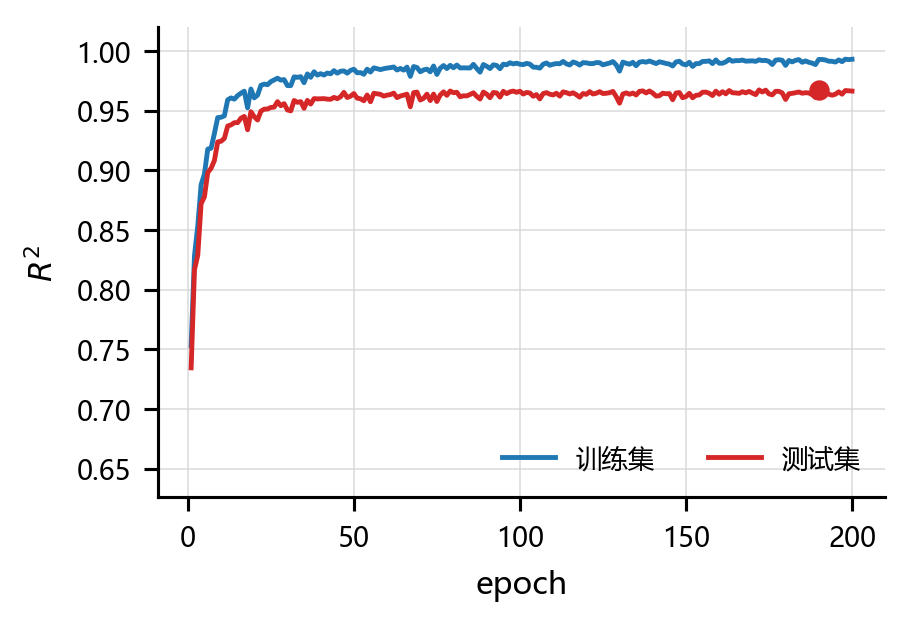
\includegraphics[width=\columnwidth]{net_train_dnn_r2_zh.png}\\[-0.2em]
{\scriptsize (a) 全量 DNN}\\[0.45em]
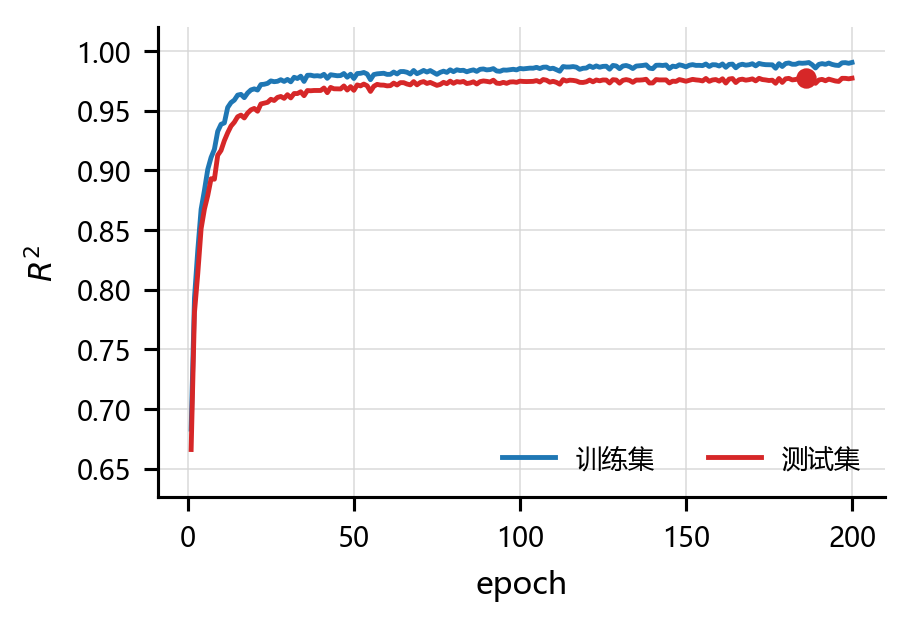
\includegraphics[width=\columnwidth]{net_train_l1_r2_zh.png}\\[-0.2em]
{\scriptsize (b) L1 门控模型}
\figbicaption{净实际交换功率目标上的 $R^2$ 训练过程对比}{Comparison of training $R^2$ processes for net actual interchange}
\label{fig:train_pair}
\end{figure}

图~\ref{fig:l1_gate} 展示了 L1 门控模型的门控参数演化过程，图中每条曲线对应一个候选字段的门控值随训练轮次的变化轨迹。在训练初期，各字段的门控值即出现明显分化；随着 L1 正则化惩罚的持续作用，大量弱贡献字段的门控值逐步衰减至阈值以下，仅有少数关键字段维持较高的门控值。在活跃阈值 $\mu_2=0.10$ 下，最终保留 18 个活跃字段，其中包含天然气发电出力、煤电出力、实时负荷、计量负荷、预估小时负荷和光伏发电出力等关键运行变量。图~\ref{fig:l1_active} 进一步展示了活跃字段数量随训练轮次的变化趋势，可以观察到活跃字段数量呈现逐步下降并趋于稳定的特征。这说明 L1 门控并非在训练结束时一次性截断弱字段，而是在优化过程中通过梯度信息逐步识别并剔除冗余字段，最终形成紧凑的推断源集合。

\begin{figure}[!tbp]
\centering

\includegraphics[width=\columnwidth]{net_l1_gate_params_zh.png}
\figbicaption{净实际交换功率目标上门控参数的演化过程}{Evolution of gate parameters for net actual interchange}
\label{fig:l1_gate}
\end{figure}

\begin{figure}[!tbp]
\centering

\includegraphics[width=\columnwidth]{net_l1_active_features_zh.png}
\figbicaption{净实际交换功率目标上活跃字段数量的变化}{Number of active features over training epochs}
\label{fig:l1_active}
\end{figure}

\subsection{Top-n 推断源验证}
为独立验证 L1 门控所选字段是否具备实际推断能力，本文按最终门控值从大到小排序，依次取 Top3、Top6、Top9、Top12、Top15、Top18 字段，分别训练普通 DNN 并评估其测试 $R^2$，同时与全量 55 字段和未选中 37 字段的结果进行比较。实验结果如图~\ref{fig:top_series} 所示。

当字段数较少时，推断能力受到明显限制：Top3 和 Top6 的测试 $R^2$ 分别仅为 0.4469 和 0.5778。随着字段数增加，推断能力显著提升：Top9 达到 0.9186，Top15 达到 0.9630，Top18 达到 0.9681，略高于全量 55 字段的 0.9661。与之形成对比的是，去除 Top18 后剩余的 37 个未选中字段单独训练仅取得 0.7820 的测试 $R^2$。上述结果表明，L1 门控识别出的字段集合具有两个重要特征：一是所选字段共同构成了支撑目标推断的核心路径，推断能力与甚至略优于全量字段；二是未选中字段尽管数量更多，但缺乏关键推断路径，单独推断能力显著下降。这进一步印证了 L1 门控不是简单挑选个别强相关字段，而是识别出能够联合支撑目标推断的非冗余字段组合。

\begin{figure}[!tbp]
\centering

\includegraphics[width=\columnwidth]{net_top_series_r2_zh.png}
\figbicaption{净实际交换功率目标上的 Top-n 推断源验证结果}{Top-n inference-source validation for net actual interchange}
\label{fig:top_series}
\end{figure}

\subsection{改进门控的风险边界学习}
图~\ref{fig:improved_gate} 至图~\ref{fig:improved_b} 展示了相关性驱动改进门控模型的训练结果。与普通 L1 门控模型不同，改进门控的门控值由六维相关性向量经 Sigmoid 映射生成，因此判定阈值设为 0.5，具有明确的数学含义：当 $W^{\mathrm{T}}R_i+b=0$ 时，Sigmoid 输出恰好为 0.5，对应风险边界；高于该边界表示相关性证据足以支持字段作为推断源，低于该边界则表示字段更可能为冗余或低风险字段。

在本次实验中，改进 L1 门控最终保留 17 个活跃字段，最优测试 $R^2$ 为 0.9726。从权重向量 $W$ 的演化过程来看，HSIC 对应的权重在训练收敛后保持最高，表明非线性依赖证据对净实际交换功率目标的风险判定贡献最为显著；偏置 $b$ 从接近零的初始值逐步下降至约 $-0.70$，反映出模型在 L1 正则化压力下不断收紧门控打开条件。改进门控的核心意义在于：它将"各类统计指标如何共同影响字段风险判定"这一问题转化为可学习的统一边界，取代了传统方法中需要为每个指标独立设置阈值的方式。

\begin{figure}[!tbp]
\centering

\includegraphics[width=\columnwidth]{improved_l1_gate_params_zh.png}
\figbicaption{改进 L1 门控模型的门控值演化}{Gate value evolution of the improved L1-gated model}
\label{fig:improved_gate}
\end{figure}

\begin{figure}[!tbp]
\centering
\begin{minipage}{\columnwidth}
\centering
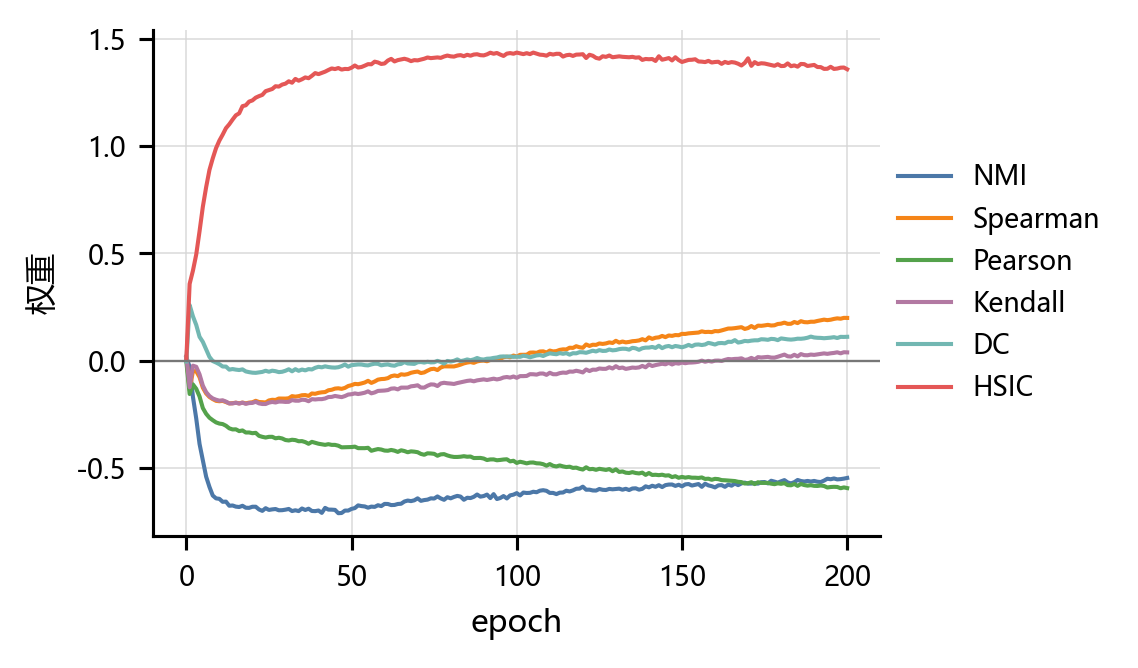
\includegraphics[width=0.92\linewidth]{improved_l1_w_meta_zh.png}\\[-0.4em]
{\scriptsize (a) 相关性指标权重 $W$ 的演化}
\end{minipage}\\[-0.2em]
\begin{minipage}{\columnwidth}
\centering

\includegraphics[width=0.86\linewidth]{improved_l1_b_meta_zh.png}\\[-0.4em]
{\scriptsize (b) 偏置 $b$ 的演化}
\end{minipage}
\figbicaption{改进门控中指标权重与偏置的训练演化}{Evolution of metric weights and bias in the improved gate}
\label{fig:improved_b}
\end{figure}

\section{多目标对比实验}
\subsection{全量模型与 L1 门控模型对比}
为系统评估所提方法的泛化性能，本文在 12 个敏感目标上开展了全量 DNN 与 L1 门控选中特征 DNN 的直接对比实验。全量 DNN 使用当前目标允许的全部候选字段进行训练，L1DNN 则先由 L1 门控模型确定活跃字段集合，再使用相同网络结构重新训练并评估。实验结果如图~\ref{fig:dnn_l1_compare} 和表~\ref{tab:dnn_l1_compare} 所示。

以数据全集中 70 个数值字段扣除目标字段后的 69 个字段作为统一全量基准，全量 DNN 的字段利用率为 100\%，12 个目标的平均测试 $R^2$ 为 0.9031；L1 门控模型平均仅使用 15.50 个字段，字段利用率约为 22.46\%，平均测试 $R^2$ 为 0.9111，高于全量 DNN 的结果。从各目标的具体表现来看，在日前拥塞价、主备用容量、总实际交换功率和净实际交换功率等目标上，L1 门控模型显著或略微优于全量 DNN；在实时拥塞价和日前 LMP 上，L1 门控模型略低于全量 DNN。上述结果表明，所提方法并非对所有目标进行机械式的字段压缩，而是能够在大多数目标上以显著缩减的字段规模保持同等甚至更优的泛化能力。对于少数字段压缩后性能略有下降的目标，其下降幅度有限，仍处于可接受范围。

\begin{figure}[!tbp]
\centering

\includegraphics[width=\columnwidth]{dnn_vs_l1_method_compare_zh.png}
\figbicaption{12 个敏感目标上全量 DNN 与 L1 门控模型的测试 $R^2$ 对比}{Comparison of test $R^2$ between all-feature DNN and L1-gated model across 12 targets}
\label{fig:dnn_l1_compare}
\end{figure}

\begin{table}[!tbp]
\centering
\scriptsize
\setlength{\tabcolsep}{2pt}
\tabbicaption{全量 DNN 与 L1 门控选中特征 DNN 的详细对比}{Detailed comparison between all-feature DNN and L1-gated selected-feature DNN}
\label{tab:dnn_l1_compare}
\begin{tabularx}{\columnwidth}{Xrrrr}
\toprule
中心目标 & 全量字段 & L1 字段 & 全量 DNN & L1DNN \\
\midrule
拥塞价 DA & 69 & 2 & 0.9408 & \textbf{0.9954} \\
主备用容量 & 67 & 14 & 0.8495 & \textbf{0.8826} \\
总实际交换 & 69 & 16 & 0.8499 & \textbf{0.8677} \\
30 min 备用容量 & 68 & 22 & 0.8967 & \textbf{0.9086} \\
边际损耗价 DA & 69 & 18 & 0.8936 & 0.8995 \\
净实际交换 & 67 & 18 & 0.9680 & 0.9728 \\
总发电量 & 42 & 16 & 0.9253 & 0.9271 \\
净计划交换 & 67 & 16 & 0.9691 & 0.9694 \\
总损耗 & 69 & 18 & 0.9413 & 0.9409 \\
计量负荷 & 42 & 15 & 0.9157 & 0.9139 \\
日前 LMP & 66 & 13 & \textbf{0.9622} & 0.9510 \\
拥塞价 RT & 69 & 18 & \textbf{0.7255} & 0.7040 \\
\midrule
平均 & -- & 15.5 & 0.9031 & 0.9111 \\
\bottomrule
\end{tabularx}
\end{table}

\subsection{同预算 baseline 对比}
为回应"baseline 的字段数 $n$ 是否由 L1 门控单方面决定"这一公平性问题，本文采用统一预算策略开展进一步对比。具体做法为：首先利用 L1 门控模型在特征预算序列上搜索，确定使其 $R^2$ 达到全量 DNN 的 95\% 或 97\% 水平时对应的字段数 $n$；若遍历候选预算后仍无法达到目标水平，则采用当前可获得的最优预算。随后，所有 baseline 方法在相同字段数 $n$ 下进行字段选择，并统一使用普通 DNN 训练和测试。在此设置下，不同方法的比较聚焦于"在相同字段预算下，谁选择的字段更具推断能力"，而非"谁使用了更多字段"。

图~\ref{fig:budget_lines} 给出了 95\% 和 97\% 统一预算下各目标的测试 $R^2$ 折线对比结果，图~\ref{fig:budget_avg} 进一步汇总了各方法在两种预算下的平均表现。在 95\% 预算水平下，平均字段数为 8.92，L1 门控模型的平均 $R^2$ 为 0.8875，高于随机森林的 0.8562、ElasticNet 的 0.8115、Lasso 的 0.7967 和 XGBoost 的 0.7798；在 97\% 预算水平下，平均字段数增加至 9.75，L1 门控模型的平均 $R^2$ 进一步提升至 0.8943，仍保持最优。在两种预算水平下，单相关性排序方法的整体表现偏低，表明仅依靠 NMI、Pearson 或 Spearman 等单一指标排序难以稳定保留联合推断所需的关键字段；树模型和线性稀疏模型虽在个别目标上具有竞争力，但在平均性能上仍不及 L1 门控模型。上述结果验证了所提方法在统一字段预算约束下的特征选择优势。

\begin{figure}[!tbp]
\centering
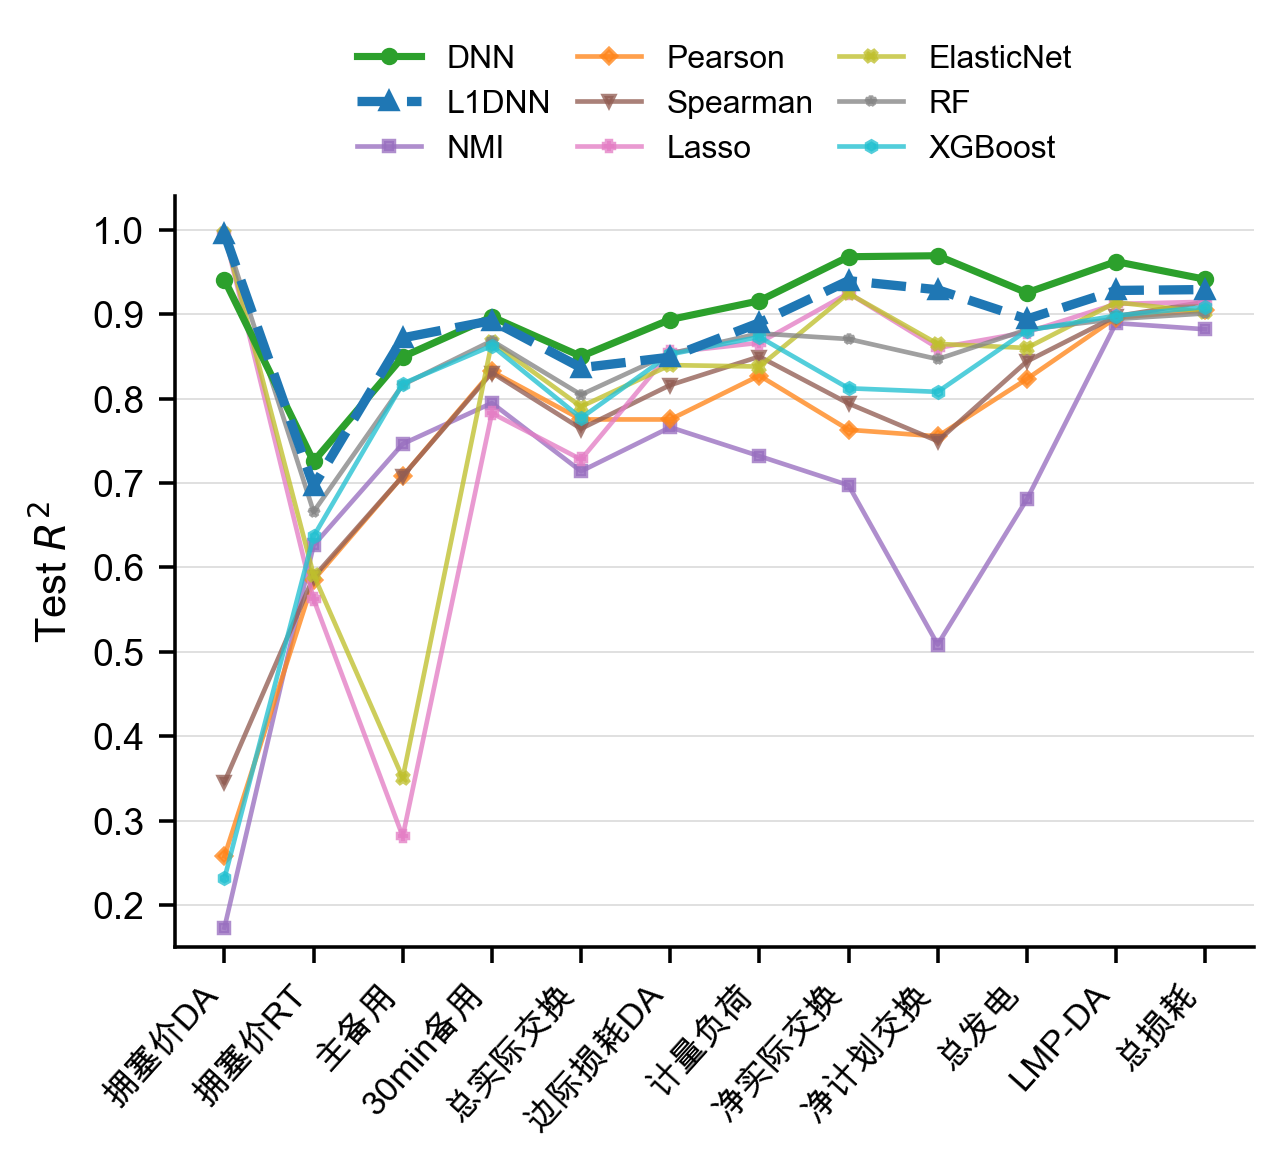
\includegraphics[width=\columnwidth]{budget95_baseline_lines_zh.png}\\[-0.2em]
{\scriptsize (a) 95\% 统一预算}\\[0.45em]
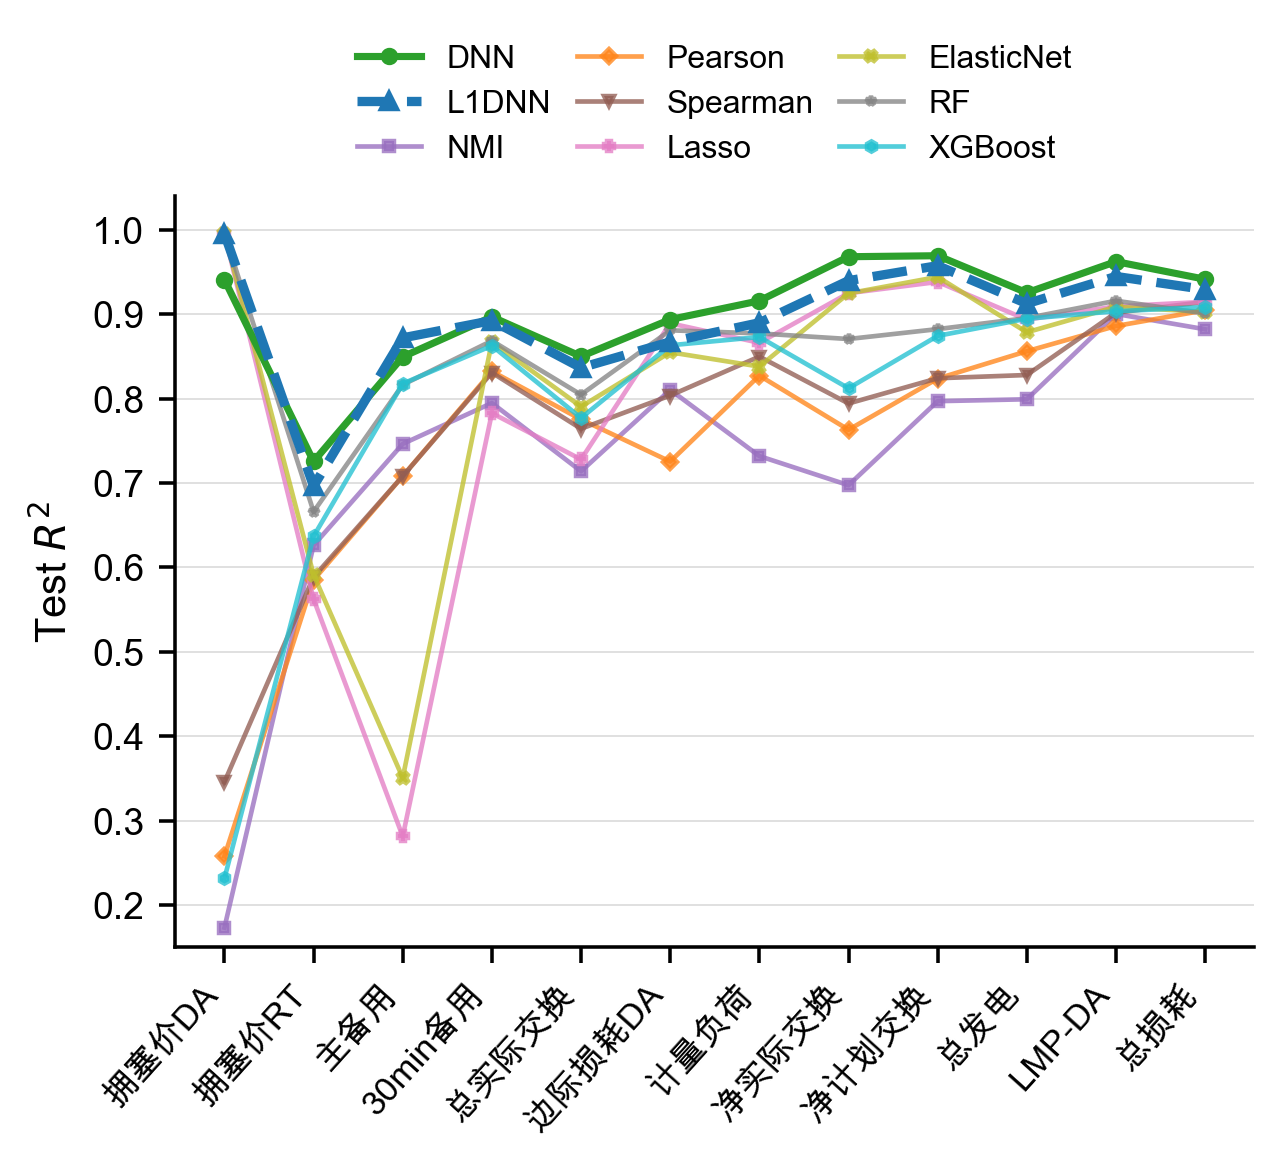
\includegraphics[width=\columnwidth]{budget97_baseline_lines_zh.png}\\[-0.2em]
{\scriptsize (b) 97\% 统一预算}
\figbicaption{统一预算下各目标的 baseline 测试 $R^2$ 对比}{Target-level baseline comparison under unified feature budgets}
\label{fig:budget_lines}
\end{figure}

\begin{figure}[!tbp]
\centering
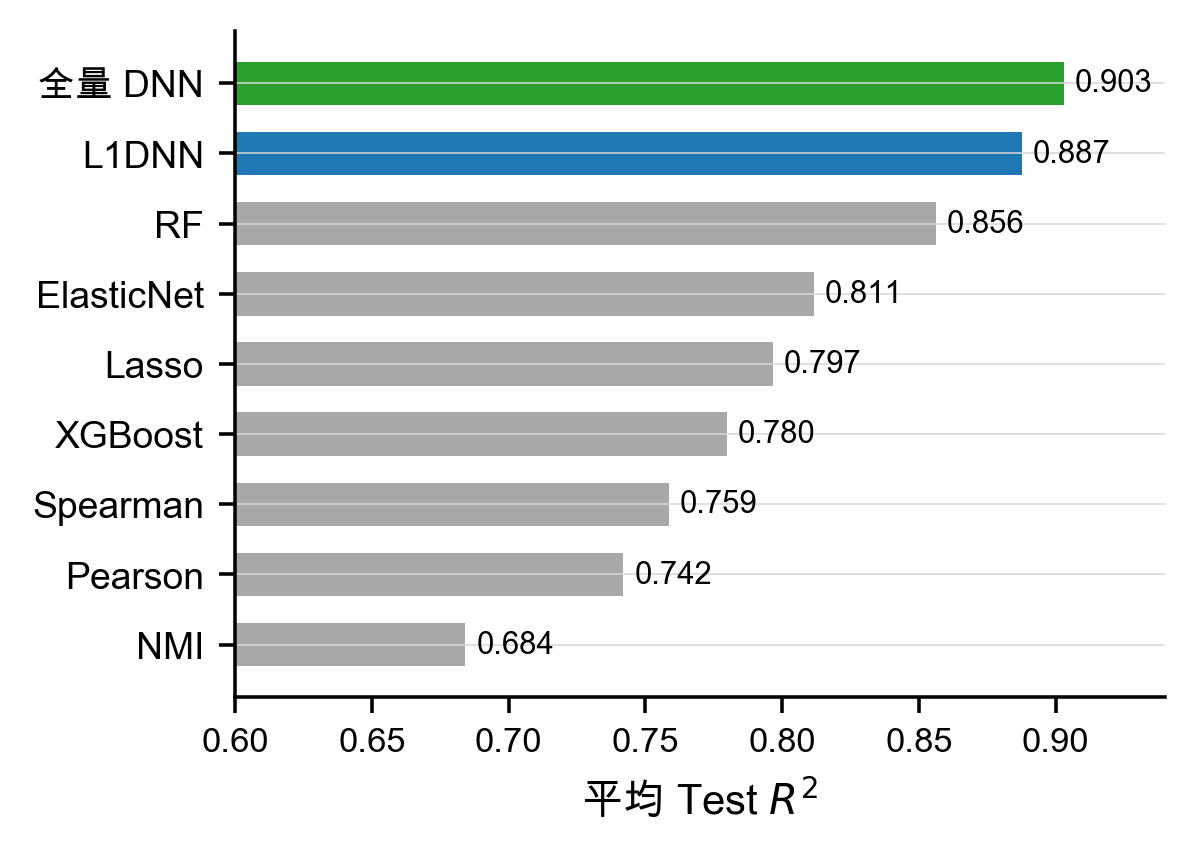
\includegraphics[width=\columnwidth]{budget95_average_bar_zh.png}\\[-0.2em]
{\scriptsize (a) 95\% 统一预算}\\[0.45em]
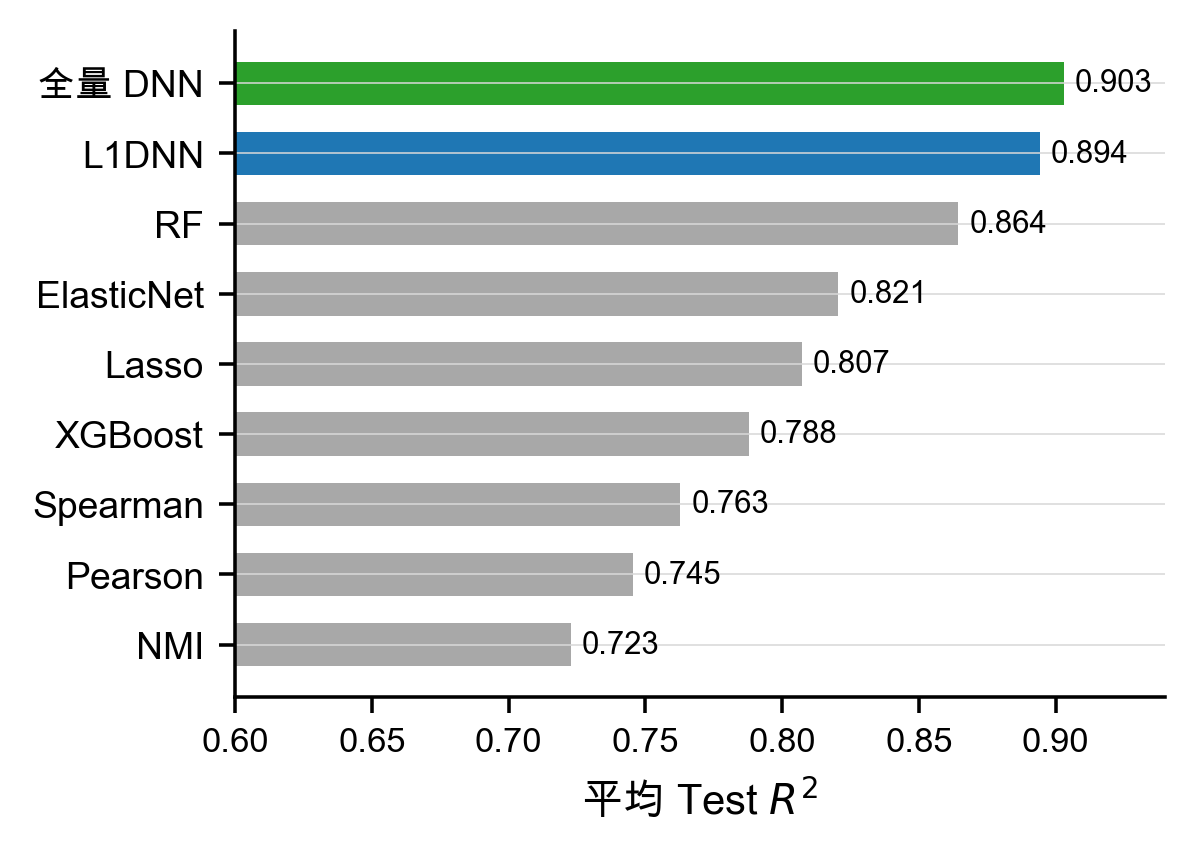
\includegraphics[width=\columnwidth]{budget97_average_bar_zh.png}\\[-0.2em]
{\scriptsize (b) 97\% 统一预算}
\figbicaption{统一预算下各 baseline 方法的平均测试 $R^2$}{Average test $R^2$ of baseline methods under unified feature budgets}
\label{fig:budget_avg}
\end{figure}

\section{冗余噪声影响分析}
\subsection{训练曲线对比分析}
在上述实验中，部分目标出现了 L1 门控选中字段的测试 $R^2$ 高于全量字段 DNN 的现象。这一看似反直觉的结果并非意味着全量字段所含信息量不足，而是揭示了全量输入中冗余和噪声字段对深度模型泛化性能的负面影响。在高维输入空间中，普通多层感知器在有限样本条件下容易对弱相关字段产生过度拟合，表现为训练集拟合度持续提升而测试集泛化性能出现下降。

为验证上述分析，本文选取性能差异较为显著的日前拥塞价和主备用容量两个目标，对比全量 DNN、L1 门控模型和 L1 选中特征再训练 DNN 的训练曲线，结果如图~\ref{fig:redundant_curve} 和表~\ref{tab:noise_curve} 所示。

对于日前拥塞价目标，全量 DNN（69 字段）的最优测试 $R^2$ 为 0.9408，最终训练集与测试集的泛化差距约为 0.0621；而仅使用 L1 门控选出的 2 个字段重新训练普通 DNN 后，最优测试 $R^2$ 达到 0.9954，泛化差距大幅缩小至 0.0025。对于主备用容量目标，全量 DNN（67 字段）的泛化差距约为 0.1439，L1 选中特征 DNN（35 字段）的测试 $R^2$ 从 0.8495 提升至 0.8580，泛化差距也有所改善。上述结果表明，字段压缩有效降低了模型对弱相关和噪声字段的过度记忆，使模型在测试集上的表现更加稳定。

\begin{figure}[!tbp]
\centering
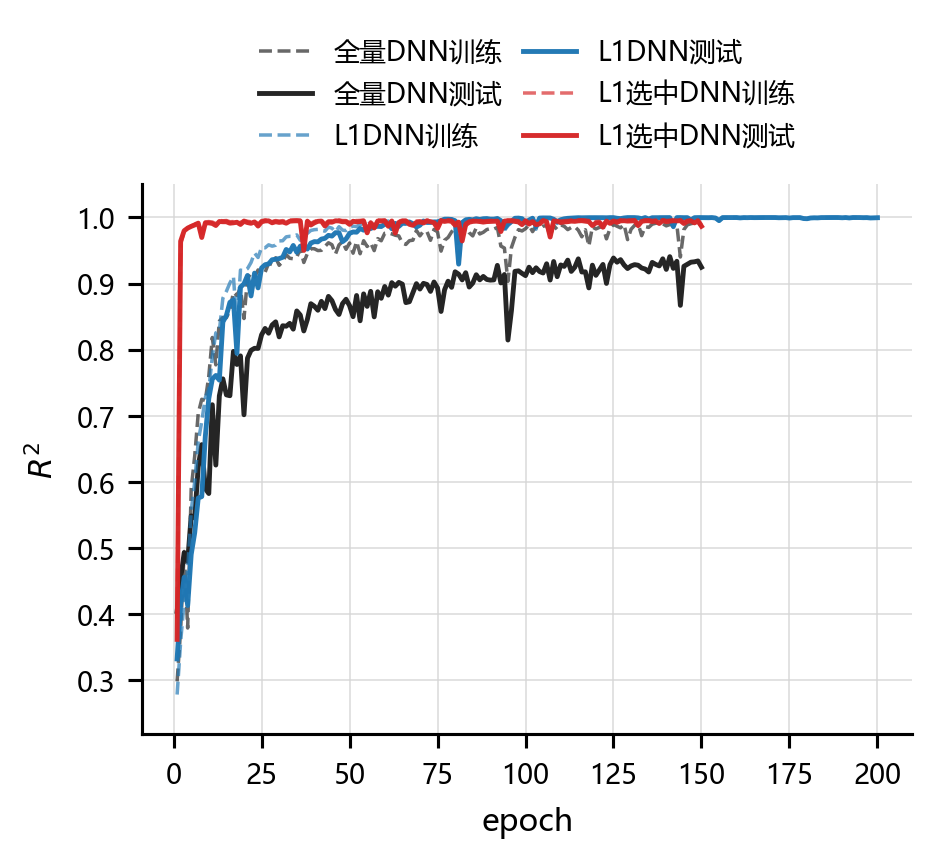
\includegraphics[width=\columnwidth]{redundant_training_congestion_zh.png}\\[-0.2em]
{\scriptsize (a) 日前拥塞价}\\[0.45em]
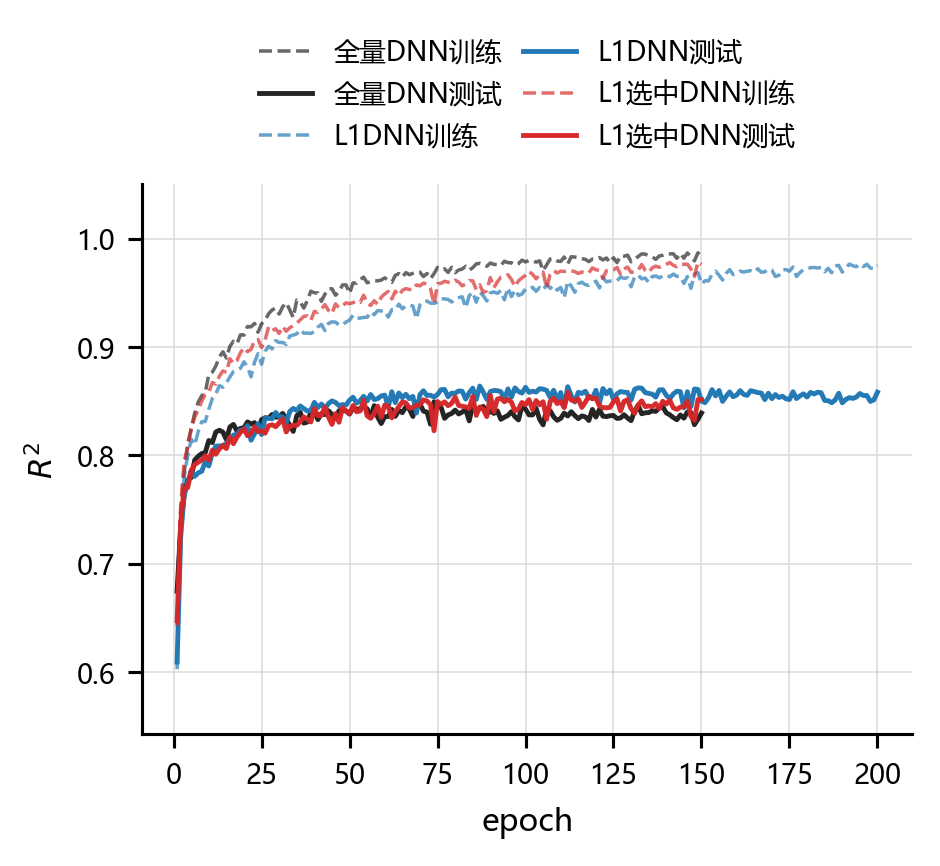
\includegraphics[width=\columnwidth]{redundant_training_primary_zh.png}\\[-0.2em]
{\scriptsize (b) 主备用容量}
\figbicaption{全量字段与 L1 选中特征的训练/测试 $R^2$ 曲线对比}{Comparison of train/test $R^2$ curves between all features and L1-selected features}
\label{fig:redundant_curve}
\end{figure}

\begin{table}[!tbp]
\centering
\scriptsize
\setlength{\tabcolsep}{3pt}
\tabbicaption{冗余噪声解释实验训练曲线统计}{Training-curve statistics for redundant-noise explanation}
\label{tab:noise_curve}
\textbf{(a) 日前拥塞价}\\[-0.2em]
\begin{tabularx}{\columnwidth}{Xrrrr}
\toprule
方法 & 字段数 & Best $R^2$ & epoch & 泛化差距 \\
\midrule
全量 DNN & 69 & 0.9408 & 141 & 0.0621 \\
L1GateDNN & 69 & 1.0000 & 194 & -0.0001 \\
L1 选中特征 DNN & 2 & 0.9954 & 139 & 0.0025 \\
\bottomrule
\end{tabularx}

\vspace{0.4em}
\textbf{(b) 主备用容量}\\[-0.2em]
\begin{tabularx}{\columnwidth}{Xrrrr}
\toprule
方法 & 字段数 & Best $R^2$ & epoch & 泛化差距 \\
\midrule
全量 DNN & 67 & 0.8495 & 74 & 0.1439 \\
L1GateDNN & 67 & 0.8639 & 87 & 0.1170 \\
L1 选中特征 DNN & 35 & 0.8580 & 112 & 0.1247 \\
\bottomrule
\end{tabularx}
\end{table}

\subsection{Top-n 递增实验}
为进一步揭示字段数量与推断性能之间的关系，本文按 L1 门控值排名逐步增加输入字段数，记录各组合下的测试 $R^2$。图~\ref{fig:topn_noise} 给出了日前拥塞价和主备用容量两个目标的完整 Top-n 序列结果，其中三角形标记表示 $R^2$ 最高点，方形标记表示全量字段对应的结果。

对于日前拥塞价目标，仅 Top2 字段即达到 0.9954 的测试 $R^2$，Top3 进一步提升至 0.9999，在 Top24 范围内均保持较高水平；然而当字段数增加至 Top32 时，$R^2$ 下降至 0.9851，全量 69 字段的结果仅为 0.9408。对于主备用容量目标，$R^2$ 随字段数从 Top1 到 Top24 逐步提升至 0.8872 的峰值，但继续增加至 Top32 和 Top35 后分别降至 0.8545 和 0.8536，接近全量 DNN 的 0.8495。

上述递增实验揭示了字段数量与推断性能之间的典型非单调关系：当关键字段不足时，模型缺乏必要的信息源，推断能力受限；当字段数量处于合理区间时，核心推断路径被充分激活，推断精度显著提升；而当冗余和弱相关字段继续加入后，输入空间的维度增大，过拟合风险相应上升，导致泛化收益递减甚至出现逆转。这一发现为数据发布场景下的字段压缩策略提供了重要启示：适度的字段删减不仅不会损害推断能力，反而可能因消除冗余噪声而提升模型的泛化表现。

\begin{figure}[!tbp]
\centering
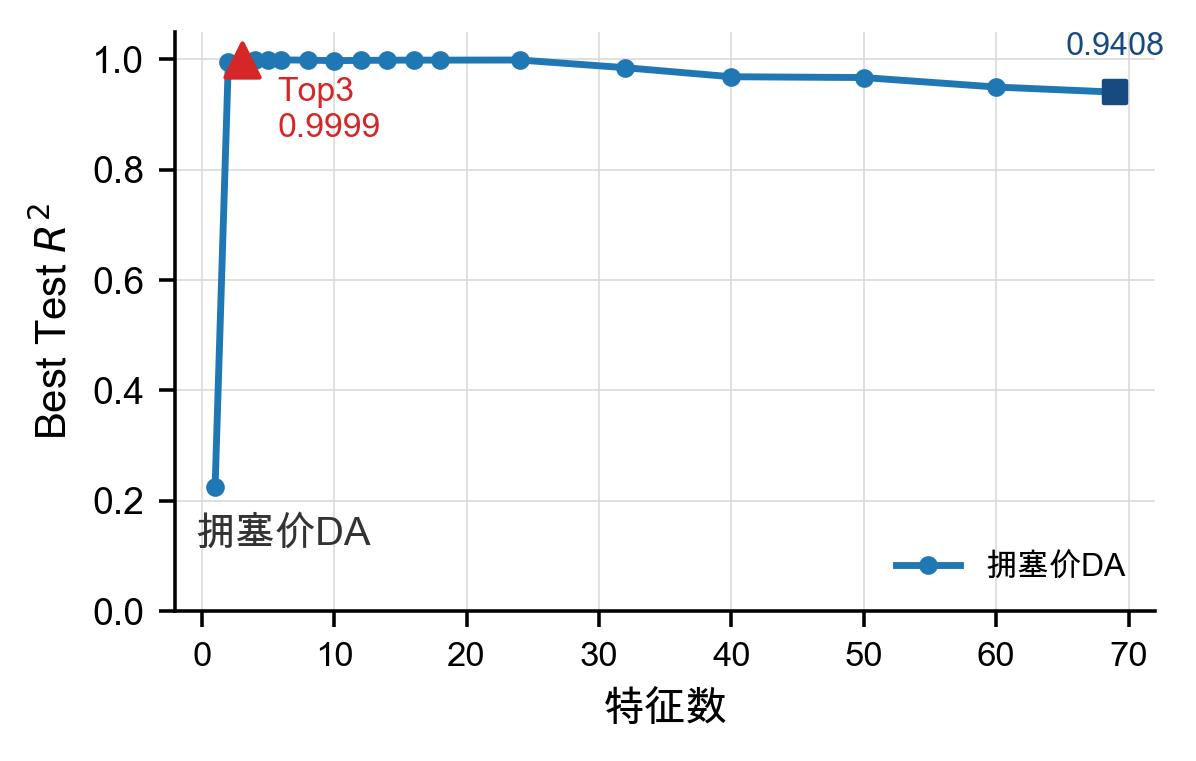
\includegraphics[width=\columnwidth]{topn_congestion_zh.png}\\[-0.2em]
{\scriptsize (a) 日前拥塞价}\\[0.45em]
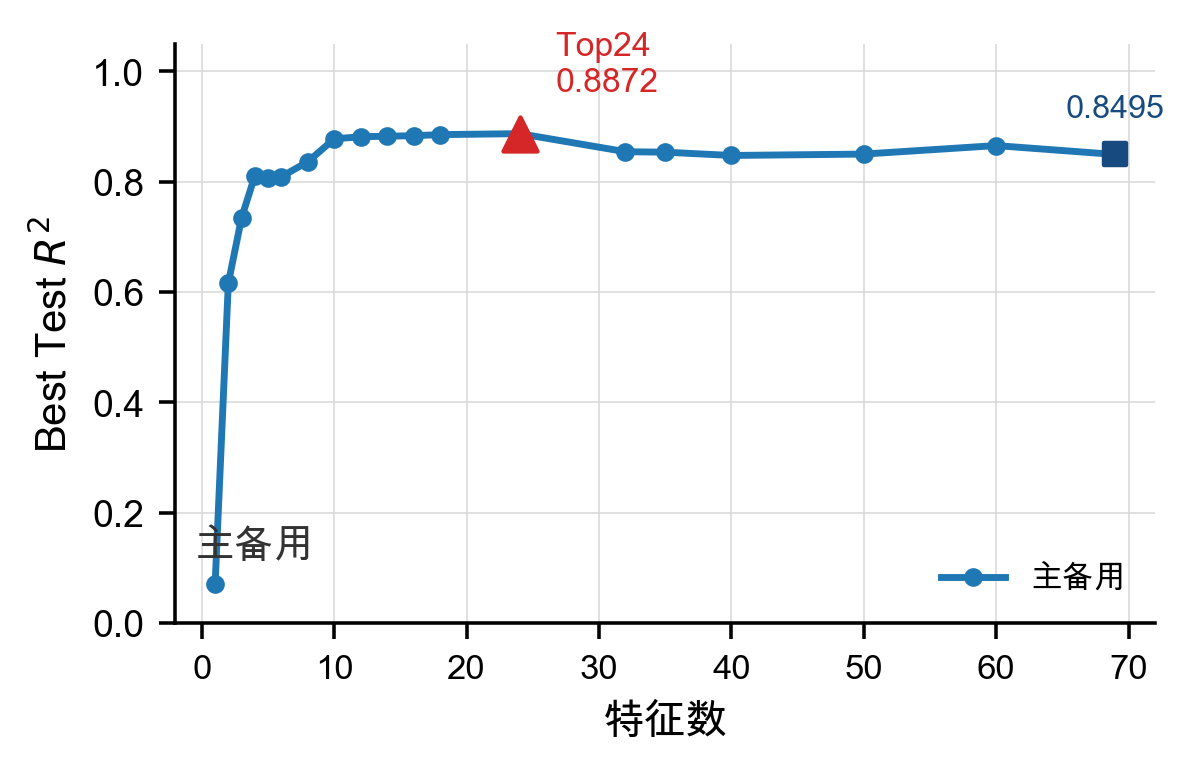
\includegraphics[width=\columnwidth]{topn_primary_zh.png}\\[-0.2em]
{\scriptsize (b) 主备用容量}
\figbicaption{按 L1 门控排名逐步增加字段数的测试 $R^2$ 变化}{Test $R^2$ variation with incrementally added Top-n features ranked by L1 gate values}
\label{fig:topn_noise}
\end{figure}

\section{讨论}
上述实验结果表明，所提 L1 门控方法的核心优势不仅体现在平均 $R^2$ 的数值提升，更在于其输出形式与电力数据发布前安全审查的实际需求高度契合。全量深度模型虽可证明敏感目标整体可被预测，但无法定位具体的推断路径和风险源字段；单相关性分析方法可以量化字段间的两两关联强度，但无法判断各字段在联合推断中的不可替代性；线性稀疏模型和树模型能够给出特征重要性排序，但其排序标准与深度模型实际推断能力之间缺乏一致性保证。本文所提 L1 门控模型将字段选择嵌入非线性深度推断的训练过程中，使字段的保留或剔除直接受到预测误差和稀疏约束的联合驱动，因此其输出的活跃字段集合更接近"哪些字段可能被攻击模型实际利用"的风险语义。

同预算 baseline 对比实验进一步说明了统一字段预算策略的合理性。固定字段数 $n$ 并非为了偏向 L1 门控方法，而是为了构造公平且可解释的比较基准：若允许各方法自由选择不同数量的字段，则性能差异可能来源于字段数差异而非选择质量差异。本文在 95\% 和 97\% 两种预算水平下均开展了对比，既展示了较低容忍度下 L1 门控方法的领先优势，也揭示了在较高容忍度下各方法性能趋近全量 DNN 的收敛趋势。

少量字段推断精度优于全量字段的现象具有深层的实际含义。在电力数据中，大量字段并非独立信息源，而是由相同的物理过程或市场机制派生而来。将这些共线性强或弱相关的字段全部作为模型输入，会扩大输入空间维度，增大深度模型记忆训练样本细节的倾向，从而加剧过拟合风险。L1 门控通过在训练过程中先行筛选出稳定推断路径，再由普通 DNN 独立验证其推断能力，实质上实现了输入维度的合理压缩和过拟合风险的有效控制。因此，字段压缩的本质并非信息舍弃，而是在保留核心推断路径的同时消除冗余噪声的干扰。

本文研究仍存在以下局限性。第一，L1 正则化系数和活跃阈值的选择会影响最终的字段筛选结果，在实际应用中应根据数据发布场景的安全等级需求进行调整。第二，部分敏感目标可能存在多条等价推断路径，单次训练得到的活跃字段集合不一定唯一，后续研究应引入多随机种子和跨时间窗口的稳定性分析机制。第三，本文以单目标推断为中心构建风险分析框架，多目标之间的联合泄露效应和风险传播机制尚待进一步研究。

\section{结论}
本文围绕电力数据共享中的隐性推断风险问题，提出了融合多相关性筛选与 L1 门控深度神经网络的分析方法。该方法首先通过六类统计指标对候选字段进行多维度依赖性初筛，确保不同类型的潜在风险字段均被保留；随后利用 L1 门控深度神经网络在保持敏感目标推断能力的前提下自动压缩冗余字段，获取紧凑的活跃推断源集合；进而通过普通深度神经网络再训练独立验证所选字段的实际推断能力。此外，本文构建的相关性驱动改进门控模型将六类统计指标映射为统一的风险判定边界，增强了分析方法的可解释性。

基于美国 PJM 电力市场 2025 年小时级运行数据的实验结果表明：针对净实际交换功率目标，所提方法从 55 个候选字段中筛选出 18 个活跃字段，以此训练的普通 DNN 验证 $R^2$ 为 0.9681，高于全量字段结果 0.9661，而未选中字段单独推断仅为 0.7820。在 12 个敏感目标上，L1 门控模型以平均 15.5 个字段（字段利用率约 22.46\%）取得 0.9111 的平均测试 $R^2$，高于全量 DNN 的 0.9031。在 95\% 和 97\% 同预算 baseline 对比中，L1 门控方法在各预算水平下均保持最优平均 $R^2$。冗余噪声影响分析进一步揭示了全量输入中弱相关和冗余字段引发过拟合的机理，为合理的字段压缩策略提供了实证依据。上述结果表明，所提方法能够有效定位电力数据中的隐性推断路径和关键风险源字段，可为数据发布前的字段安全审查、敏感等级评估和推断路径阻断提供技术支撑。

未来研究将从以下三个方面展开：一是引入多随机种子和跨月份时间窗口验证，评估门控字段集合的跨场景稳定性；二是将单目标推断分析扩展为多目标风险图谱构建，系统刻画不同敏感字段之间的联合泄露关系和风险传播路径；三是将识别出的风险源集合与字段降精度、延迟发布和分级授权等数据处置策略相结合，构建面向实际电力数据共享流程的闭环安全防护机制。

\balance
\begin{thebibliography}{99}
\bibitem{ref-liu-cps}
刘涛, 田捷, 王杰, 等. 信息物理融合系统的综合安全威胁与防御研究[J]. 自动化学报, 2019, 45(1): 5-24.

LIU Tao, TIAN Jie, WANG Jie, et al. Integrated security threats and defense of cyber-physical systems[J]. Acta Automatica Sinica, 2019, 45(1): 5-24.

\bibitem{ref-ma-pjm}
马珍, 张弘, 朱兰, 等. 美国电力市场信息披露制度及其对中国的启示[J]. 电力系统自动化, 2017, 41(24): 49-57.

MA Zhen, ZHANG Hong, ZHU Lan, et al. Information disclosure system in American electricity market and its enlightenment for China[J]. Automation of Electric Power Systems, 2017, 41(24): 49-57.

\bibitem{ref-fan-pjm}
Fan Z, Horger T, Bastian J, et al. An overview of PJM energy market design and development[C]//2008 Third International Conference on Electric Utility Deregulation and Restructuring and Power Technologies. Piscataway: IEEE, 2008: 12-17.

\bibitem{ref-sankar}
Sankar L, Rajagopalan S R, Mohajer S, et al. Smart meter privacy: A theoretical framework[J]. IEEE Transactions on Smart Grid, 2013, 4(2): 837-846.

\bibitem{ref-giaconi}
Giaconi G, Gündüz D, Poor H V. Privacy-aware smart metering: Progress and challenges[J]. IEEE Signal Processing Magazine, 2018, 35(6): 59-78.

\bibitem{ref-adewole}
Adewole K S, Torra V. Privacy issues in smart grid data: From energy disaggregation to disclosure risk[C]//International Conference on Database and Expert Systems Applications. Cham: Springer, 2022: 71-84.

\bibitem{ref-lan-load}
兰丁, 朱慧, 吴杰, 等. 基于改进 AlexNet-GRU 深度学习网络的配电网短期负荷预测方法[C]//2021 IEEE 5th Conference on Energy Internet and Energy System Integration. Piscataway: IEEE, 2021: 3004-3010.

LAN Ding, ZHU Hui, WU Jie, et al. A short-term load forecasting method of distribution network based on improved AlexNet-GRU deep learning network[C]//2021 IEEE 5th Conference on Energy Internet and Energy System Integration. Piscataway: IEEE, 2021: 3004-3010.

\bibitem{ref-jiao-pv}
焦鑫, 孙源, 彭迪, 等. 基于方差变点与相关性分析的光伏功率异常数据清洗[C]//2021 6th International Conference on Power and Renewable Energy. Piscataway: IEEE, 2021: 1140-1145.

JIAO Xin, SUN Yuan, PENG Di, et al. Photovoltaic power abnormal data cleaning based on variance change point and correlation analysis[C]//2021 6th International Conference on Power and Renewable Energy. Piscataway: IEEE, 2021: 1140-1145.

\bibitem{ref-deng-load}
邓鑫, 张超, 彭辉, 等. 基于相关性分析与特征提取的区域电网短期负荷预测[C]//2022 7th Asia Conference on Power and Electrical Engineering. Piscataway: IEEE, 2022: 1081-1085.

DENG Xin, ZHANG Chao, PENG Hui, et al. Short-term load forecasting for regional power grids based on correlation analysis and feature extraction[C]//2022 7th Asia Conference on Power and Electrical Engineering. Piscataway: IEEE, 2022: 1081-1085.

\bibitem{ref-szekely-dcorr}
Székely G J, Rizzo M L, Bakirov N K. Measuring and testing dependence by correlation of distances[J]. The Annals of Statistics, 2007, 35(6): 2769-2794.

\bibitem{ref-gretton-hsic}
Gretton A, Bousquet O, Smola A, et al. Measuring statistical dependence with Hilbert-Schmidt norms[C]//Algorithmic Learning Theory. Berlin: Springer, 2005: 63-77.

\bibitem{ref-wang-meter}
Wang Y, Chen Q, Hong T, et al. Review of smart meter data analytics: Applications, methodologies, and challenges[J]. IEEE Transactions on Smart Grid, 2019, 10(3): 3125-3148.

\bibitem{ref-breiman-rf}
Breiman L. Random forests[J]. Machine Learning, 2001, 45(1): 5-32.

\bibitem{ref-chen-xgboost}
Chen T, Guestrin C. XGBoost: A scalable tree boosting system[C]//Proceedings of the 22nd ACM SIGKDD International Conference on Knowledge Discovery and Data Mining. New York: ACM, 2016: 785-794.

\bibitem{ref-tibshirani-lasso}
Tibshirani R. Regression shrinkage and selection via the lasso[J]. Journal of the Royal Statistical Society: Series B, 1996, 58(1): 267-288.

\bibitem{ref-zou-enet}
Zou H, Hastie T. Regularization and variable selection via the elastic net[J]. Journal of the Royal Statistical Society: Series B, 2005, 67(2): 301-320.

\bibitem{ref-xing-micdnn}
邢治, 王征, 冯健, 等. MIC-DNN：电力数据关联分析框架[C]//2025 40th Youth Academic Annual Conference of Chinese Association of Automation. Piscataway: IEEE, 2025: 2969-2974.

XING Zhi, WANG Zheng, FENG Jian, et al. MIC-DNN: Data-driven correlation analysis framework for power data[C]//2025 40th Youth Academic Annual Conference of Chinese Association of Automation. Piscataway: IEEE, 2025: 2969-2974.

\bibitem{ref-zhang-sgcc}
张伯明, 孙宏斌, 吴文传, 等. 智能电网控制中心的信息安全问题[J]. 南方电网技术, 2012, 6(2): 1-7.

ZHANG Boming, SUN Hongbin, WU Wenchuan, et al. Information security issues in smart grid control centers[J]. Southern Power System Technology, 2012, 6(2): 1-7.

\bibitem{ref-chen-privacy}
陈颖, 王科, 朱涛, 等. 电力大数据隐私保护技术综述[J]. 电力系统自动化, 2021, 45(14): 157-168.

CHEN Ying, WANG Ke, ZHU Tao, et al. Review on privacy-preserving technologies for power big data[J]. Automation of Electric Power Systems, 2021, 45(14): 157-168.

\bibitem{ref-lecun-deep}
LeCun Y, Bengio Y, Hinton G. Deep learning[J]. Nature, 2015, 521(7553): 436-444.

\bibitem{ref-goodfellow-deep}
Goodfellow I, Bengio Y, Courville A. Deep learning[M]. Cambridge: MIT Press, 2016.

\bibitem{ref-he-dropout}
Srivastava N, Hinton G, Krizhevsky A, et al. Dropout: A simple way to prevent neural networks from overfitting[J]. The Journal of Machine Learning Research, 2014, 15(1): 1929-1958.

\bibitem{ref-kingma-adam}
Kingma D P, Ba J. Adam: A method for stochastic optimization[C]//International Conference on Learning Representations. San Diego: ICLR, 2015.

\bibitem{ref-reshef-mic}
Reshef D N, Reshef Y A, Finucane H K, et al. Detecting novel associations in large data sets[J]. Science, 2011, 334(6062): 1518-1524.

\bibitem{ref-cover-info}
Cover T M, Thomas J A. Elements of information theory[M]. 2nd ed. Hoboken: John Wiley \& Sons, 2006.

\bibitem{ref-pjm-dataminer}
PJM Interconnection. PJM Data Miner 2[EB/OL]. [2025-05-01]. https://dataminer2.pjm.com.

\bibitem{ref-zhu-sharing}
朱涛, 陈颖, 张宁, 等. 面向电力数据共享的安全机制研究[J]. 中国电机工程学报, 2020, 40(S1): 21-30.

ZHU Tao, CHEN Ying, ZHANG Ning, et al. Security mechanisms for power data sharing[J]. Proceedings of the CSEE, 2020, 40(S1): 21-30.
\end{thebibliography}

\section*{收稿日期与作者简介}
\noindent\textbf{收稿日期：}20XX-XX-XX

\noindent\textbf{作者简介：}\par
\noindent 杜浩存（出生年），男，研究方向为电力数据安全、信息物理系统安全与机器学习安全，邮箱：待补充。

\end{document}
